
\newpage{\ } 
\thispagestyle{empty} 

\chapter{Procesamiento de im\'agenes satelitales}
\lhead{Capítulo 3. \emph{Procesamiento de im\'agenes satelitales}} % This is for the header on each page - perhaps a shortened title
La teledetecci\'on presenta un principio base similar al de la visi\'on, permitiendo mediante una fuente de energ\'ia, un objetivo o escena y un sensor, generar im\'agenes digitales que posibilitan resaltar aquellos elementos dif\'iciles de percibir o ser distinguidos directamente a trav\'es de una imagen normal. A todo esto sum\'andole el comportamiento caracter\'istico que poseen los recursos naturales a sensores espaciales, nos posibilita el empleo amplio de t\'ecnicas de procesamiento de im\'agenes provechosos para el logro de los objetivos en la investigaci\'on. Este capitulo consiste en brindar conceptos espec\'ificos utilizados por la metodolog\'ia, posibilitando comprender la influencia de cada factor en el empleo de im\'agenes satelitales para la estimaci\'on de p\'erdida del contenido de carbono forestal.

\section{Sensores Remotos}
Los sensores remotos nos permiten obtener informaci\'on de la superficie terrestre, soportados en diferentes plataformas (terrestre, \'area y satelital), mediante la captura de energ\'ias reflejadas o radiadas proveniente del sol (sensores pasivos) o del mismo sensor (sensores activos) para luego ser transformadas en productos con diversos y diferentes especificaciones, siendo fotografi\'as \'areas e im\'agenes de sat\'elites los m\'as conocidos.
\subsection{El espectro electromagn\'etico}
A pesar de que las longitudes de ondas son continuas, se establece un serie de bandas donde las radiaciones manifiestan un comportamiento similar organizando las de este modo, en un espectro electromagn\'etico\cite{remote2010abdulrahman}.
Las bandas m\'as empleadas son las siguientes\cite{salinero2002teledeteccion}:
	\begin{itemize}
		\item \textbf{Espectro visible:} (400 nm a 700 nm) se denomina as\'i por tratarse de la \'unica radiaci\'on electromagn\'etica que pueden percibir nuestros ojos, coincidiendo con las longitudes de onda en donde es m\'axima la radiaci\'on solar. Dentro de esta se distinguen tres bandas fundamentales: Azul (400 nm a 500 nm), verde (500 nm a 600 nm) y rojo (600 nm a 700 nm).
		\item \textbf{Infrarrojo pr\'oximo:} (700 nm a 1300 nm) se utiliza para discriminar masas vegetales y concentraciones de humedad.
		\item \textbf{Infrarrojo medio:} (1,3 um a 8 um) en esta franja se entremezclan los procesos de reflexi\'on de la luz solar y de emisi\'on de la superficie terrestre. Se utiliza para estimar contenido de humedad en la vegetaci\'on y los focos de alta temperatura.
		\item \textbf{Infrarrojo lejano o térmico:} (8 um a 14 um) se detecta el calor de la mayor\'ia de las cubiertas terrestres.
		\item \textbf{Microondas:} (a partir de 1 um) de gran inter\'es por ser un tipo de energ\'ia transparente a la cubierta nubosa.
	\end{itemize}

\subsection{Firmas espectrales}
Las firmas espectrales consisten en la represntaci\'on de energ\'ia reflejada con relaci\'on a las longitudes de ondas, consideradas sin el efecto atmosf\'erico y medida en condiciones ideales del \'angulo incidente. Ayudan a identificar los objetos en la superficie terrestre debido a que cada uno presenta una respuesta espectral \'unica\cite{sivakumar2004satellite}.\\~\\
En la siguiente figura se observa como cada objeto difiere de los dem\'as en sus firmas espectrales:

\begin{figure}[!hbtp]
	\centering
	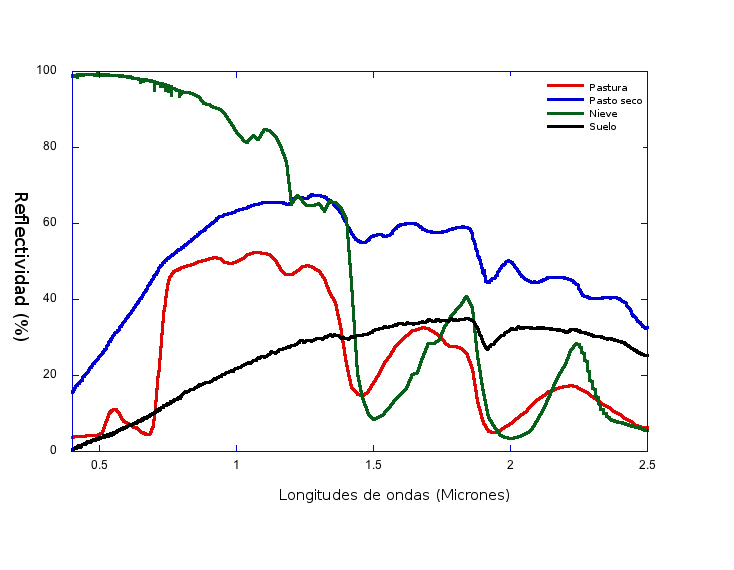
\includegraphics[width=0.9	\textwidth]{./Figures/cap3/firmaEspectral.jpg}
	\caption{Firmas espectrales de diferentes coberturas.}
	\label{fig:firmaEspectral}
\end{figure}

\subsection{Resoluciones de un sensor}

Se define a la resoluci\'on de un sensor como el menor cambio en la magnitud de entrada que puede ser apreciada en la magnitud de salida. El concepto de resoluci\'on implica al menos cuatro manifestaciones \cite{peralta2013analisis}: 
	\begin{itemize}
		
		\item \textbf{Resolución espacial:} Es el tamaño que representa en el terreno una unidad de pixel de la imagen. Tiene mucha importancia en la interpretaci\'on pues marca el nivel de detalle que ofrece, cuanto menor sea el tama\~{n}o del pixel, menor ser\'a tambi\'en la probabilidad de que corresponda a un compuesto de dos o m\'as \'areas fronterizas.
		\begin{figure}[H]
			\centering
			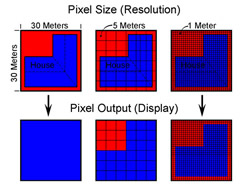
\includegraphics[width=0.4	\textwidth]{./Figures/cap3/espatialRes.jpg}
			\caption{Resoluci\'on espacial.}
			\label{fig:espatialRes}
		\end{figure}
		\item \textbf{Resoluci\'on espectral:} Indica el n\'umero y anchura de las bandas espectrales que puede discriminar el sensor. Un sensor ser\'a tanto m\'as id\'oneo cuanto mayor n\'umero de bandas proporcione, ya que facilita la caracterizaci\'on espectral de las distintas cubiertas.
				\begin{figure}[H]
					\centering
					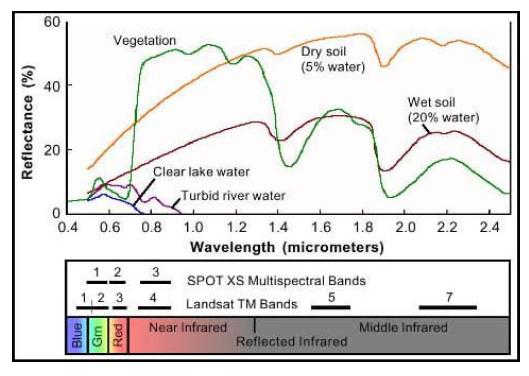
\includegraphics[width=0.6	\textwidth]{./Figures/cap3/resolucionespectral.jpg}
					\caption{Resoluci\'on espectral igual a 3 para el sensor SPOT y 7 en el sensor Landsat.}
					\label{fig:espectralRes}
				\end{figure}
		\item \textbf{Resoluci\'on radiom\'etrica:} Es la sensibilidad del sensor para detectar variaciones en la cantidad de energ\'ia espectral recibida. La sensibilidad se expresa en bits e indica el n\'umero de los distintos niveles radiom\'etricos que puede detectar un sensor.
						\begin{figure}[H]
							\centering
							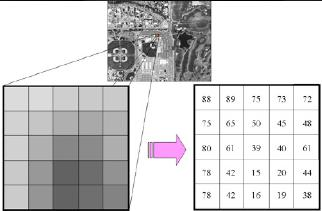
\includegraphics[width=0.6	\textwidth]{./Figures/cap3/resolucionradiometrica.jpg}
							\caption{Resoluci\'on radiom\'etrica de 8 bits (0 a 255 niveles digitales).}
							\label{fig:radioRes}
						\end{figure}
		\item \textbf{Resoluci\'on temporal:} Este tipo de resoluci\'on se refiere al intervalo de tiempo entre muestras sucesivas de la misma zona de la cobertura terrestre. El ciclo de cobertura est\'a en funció\'on de las caracter\'isticas orbitales de la plataforma, su velocidad, el ancho de barrido del sensor y las caracter\'isticas de construcci\'on del sistema.
			\begin{figure}[H]
					\centering
					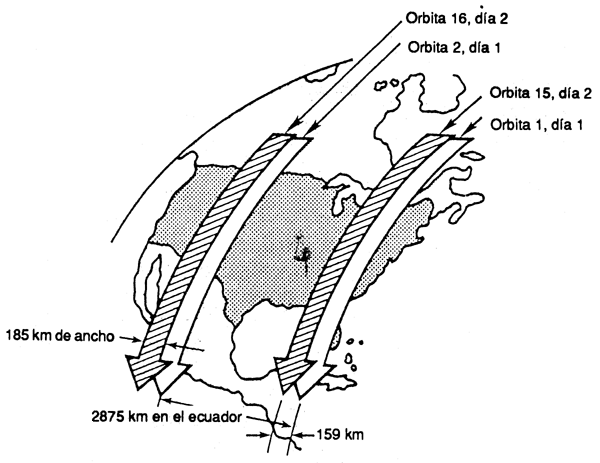
\includegraphics[width=0.6	\textwidth]{./Figures/cap3/temporalRes.png}
					\caption{Resoluci\'on temporal de 16 d\'ias.}
					\label{fig:temporaRes}
				\end{figure}
		

		
	\end{itemize}

\section{Im\'agenes satelitales}
Una imagen satelital o imagen de sat\'elite se puede definir como la representaci\'on visual de la informaci\'on capturada por un sensor montado en un sat\'elite artificial. Est\'an organizados en un arreglo matricial bidimensional de elementos llamados p\'ixeles, donde cada p\'ixel representa un \'area de superficie sobre la tierra con un valor de intensidad y una ubicación en la imagen, tambi\'en son conocidas como im\'agenes r\'aster \cite{acosta2003experiencia}. 

\subsection{Tipo de im\'agenes satelitales}
Las im\'agenes satelitales se dividen en dos tipos \cite{salinero2002teledeteccion}:
	\begin{itemize}
		\item \textbf{Pancrom\'aticas:} se captan mediante un sensor digital que mide la reflectancia de energ\'ia en una amplia parte del espectro electromagn\'etico. Para los sensores pancrom\'aticos m\'as modernos, esta \'unica banda suele abarcar la parte visible e infrarrojo cercano del espectro. Los datos pancrom\'aticos se representan por medio de im\'agenes en blanco y negro. 
		\item \textbf{Multiespectrales:} se captan mediante un sensor digital que mide la reflectancia en muchas bandas. Por ejemplo, un conjunto de detectores puede medir energ\'ia roja reflejada dentro de la parte visible del espectro mientras que otro conjunto mide la energ\'ia del infrarrojo cercano. Es posible incluso que dos series de detectores midan la energ\'ia en dos partes diferentes de la misma longitud de onda. Estos distintos valores de reflectancia se combinan para crear im\'agenes de color.

	\end{itemize}
	
\section{\'Indices de vegetaci\'on}
Los \'indices de vegetaci\'on son transformaciones que implican efectuar una combinaci\'on matem\'atica, entre los niveles digitales almacenados en dos o m\'as bandas espectrales de la misma imagen, teniendo en cuenta el comportamiento radiom\'etrico de la vegetaci\'on vigorosa para la elecci\'on de bandas\cite{speranza2005potencialidad}. \\~\\
El estudio de las cubiertas vegetales mediante la teledetecci\'on se aborda tradicionalmente mediante la utilización de los denominados “índices de vegetaci\'on”, el índice de vegetaci\'on m\'as utilizado es el NDVI (\'Indice de vegetaci\'on diferencial normalizada)\cite{sader2000estimacion}.

\subsection{\'Indice de vegetaci\'on diferencial normalizada}
Es un \'indice usado para estimar la cantidad, calidad y desarrollo de la vegetaci\'on, por medio de sensores remotos instalados com\'unmente desde la plataforma espaciales, es decir mide las condiciones de vigor vegetal de la planta, principalmente su contenido en clorofila\cite{salinero2002teledeteccion}. El objetivo del NDVI es la reducci\'on de m\'ultiples bandas a una sola, condensando la informaci\'on m\'as importante, en este caso la vegetaci\'on.\\~\\
Chuvieco\cite{salinero2002teledeteccion} menciona que la principal ventaja del NDVI es su f\'acil interpretaci\'on, ya que sus
valores var\'ian entre -1 y +1 permitiendo conocer el estado de vigor vegetal en grandes superficies, detectando fen\'omenos de amplio rango.\\~\\
Se calcula extrayendo de las bandas correspondientes al rojo $B_{R}$ e infrarrojo pr\'oximo $B_{IRc}$ seg\'un la siguiente expresi\'on:
	\begin{equation}
	NDVI=\dfrac{B_{IRc}-B_{R}}{B_{IRc}+B_{R}}
	\end{equation}
Las plantas muestran un fuerte pico de absorci\'on causados por los pigmentos fotosint\'eticos en longitudes de onda cercanas a los 700 micrones, hecho que contrasta con una fuerte reflexi\'on de las longitudes de onda del infrarrojo cercano. Por su parte, los suelos desnudos se caracterizan por un incremento suavemente monot\'onico de la reflectancia, a medida que aumenta la longitud de onda.

\section{An\'alisis Multitemporal}
Sea uno u otro el enfoque aplicado al estudio multitemporal, resulta preciso abordar previamente una serie de tratamientos sobre las im\'agenes satelitales de cara a garantizar su comparabilidad. Existen factores que influye desde la captura de informaci\'on hasta su transformaci\'on a niveles digitales.

%\begin{equation}
%\label{eq:imagenDigital}
%f(i,j)=\begin{bmatrix}
%f(0,0) &f(0,1)  & \cdots & f(0,N-1) \\ 
%f(1,0) & f(1,1) & \cdots  & f(1,N-1)\\ 
 %\vdots & \vdots & & \vdots \\ 
 %f(M-1,0) & f(M-1,1)  &\cdots  & f(M-1,N-1)
%\end{bmatrix}
%\end{equation}




 %\begin{figure}[H]
%	\centering
%		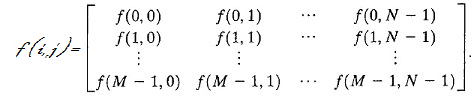
\includegraphics[width=0.7	\textwidth]{./Figures/cap3/id2.png}
%	\caption{Representación de una imagen digital.}
%	\label{fig:green}
%\end{figure}
%\nomenclature[1]{$f$}{Función que representa una imagen digital.}%
%\nomenclature[2]{$f(i,j)$}{Intensidad del píxel de la fila $i$ y columna $j$ de la imagen digital.}%
%\nomenclature[2]{$(i,j)$}{Píxel en la la fila $i$ y columna $j$  de la imagen.}%


%\subsection{Canal Verde}
%Debido a que la mayoría de los algoritmos de visión por computadora se llevan a cabo utilizando imágenes monocromáticas (binarias y en escalas de grises) \cite{gonzalezdigital,gonzales2002digital}, además de los parámetros a color $RGB$ no son necesarios en nuestra clasificación, se decidió convertir la imagen $RGB$ en una imagen en escala de grises, como se muestra en la FIGURA \ref{fig:green}.

%La conversión del espacio de color también se puede realizar en cada uno de los planos de una imagen a color $RGB$, en este caso se hace con la conversión con el canal Verde.

  %\begin{figure}[H]
%	\centering
%		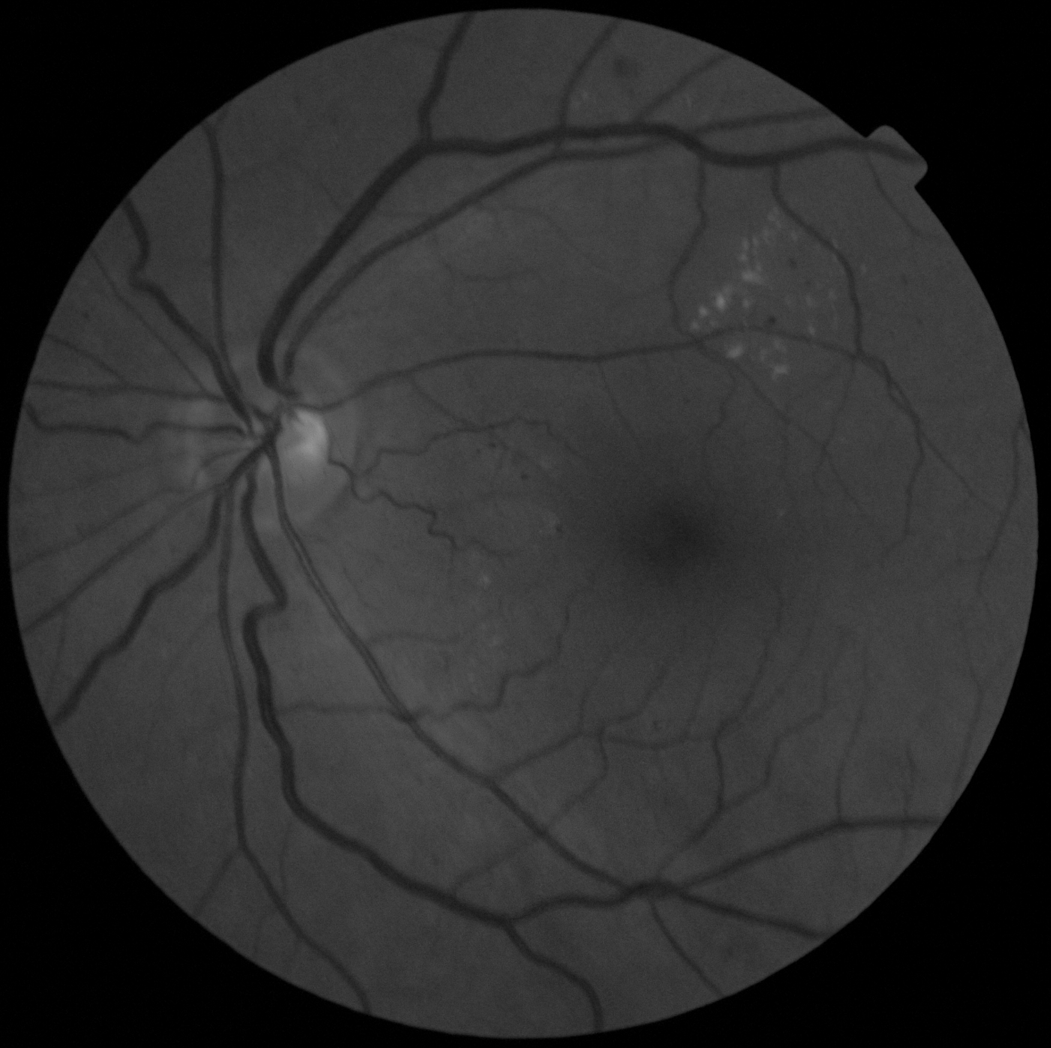
\includegraphics[width=0.4	\textwidth]{./Figures/greenChannel.png}
%	\caption{Canal Verde}
%	\label{fig:green}
%\end{figure}

